% This is text associated with the open textbook "Open Electromagnetics"
% See immediately below for author, date
% This work is licensed under the Creative Commons Attribution-ShareAlike 4.0 International License. (CC BY-SA 4.0) 
% To view a copy of the license, visit http://creativecommons.org/licenses/by-sa/4.0/

%ORB TITLE Magnetic Field of an Infinite Current Sheet
%ORB AUTHOR 0        # S.W. Ellingson, Virginia Tech (ellingson@vt.edu)
%ORB DATE 20180628   # yyyymmdd
%ORB ABSTRACT Magnetic Field of an Infinite Current Sheet

\label{m0121_Magnetic_Field_of_an_Infinite_Current_Sheet} % <-- Must match name of this file and module directory name.  Don't mess with this!

We now consider the magnetic field due to an infinite sheet of current, 
\index{current density!surface}
shown in Figure~\ref{m0121_fCurrentSheet}.
The solution to this problem is useful as a building block and source of insight in more complex problems, as well as being a useful approximation to some practical problems involving current sheets of finite extent including, for example, microstrip transmission line and ground plane currents in printed circuit boards.
%
\begin{figure}[b!]
\begin{center}
\pdftooltip{{  % note double braces
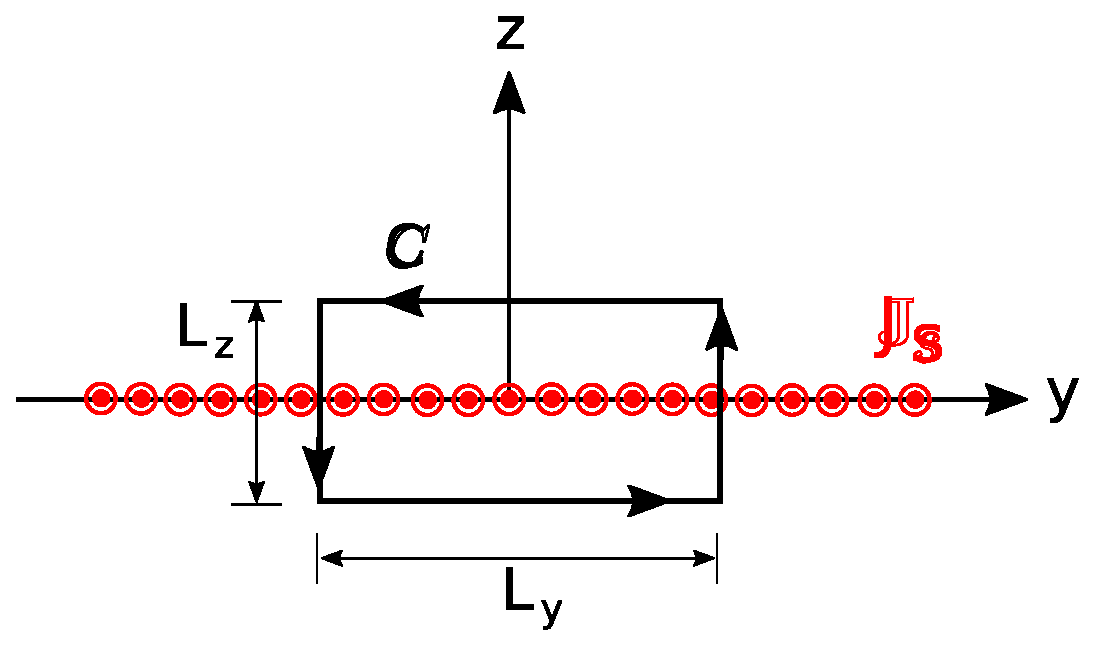
\includegraphics[width=\columnwidth]{modules/m0121_fCurrentSheet.eps}
}}{A rectangle in a closed loop, C, with counterclockwise direction. The z-axis projects perpendicularly from the center of the closed path. Along the y-axis, which runs horizontally through the closed path are red circles with red dots inside labeled J sub s. The closed path has length L sub y and height L sub z. }
\end{center} 
% URL
%\centerline{\scriptsize 
%\copyright~\hyperref[m0121_fCurrentSheet_Credit]{Slick} 
%\href{https://creativecommons.org/publicdomain/zero/1.0/deed.en}{CC0 1.0} 
%} 
\caption{
\label{m0121_fCurrentSheet}
Analysis of the magnetic field due to an infinite thin sheet of current.
}
\end{figure} 

The current sheet in Figure~\ref{m0121_fCurrentSheet} lies in the $z=0$ plane and the current density is ${\bf J}_s = \hat{\bf x}J_s$ (units of A/m); i.e., the current is uniformly distributed such that the total current crossing any segment of width $\Delta y$ along the $y$ direction is $J_s \Delta y$.

To begin, let's take stock of what we already know about the answer, which is actually quite a bit.
For example, imagine the current sheet as a continuum of thin strips parallel to the $x$ axis and very thin in the $y$ dimension.  
Each of these strips individually behaves like a straight line current $I=J_s\Delta y$ (units of A).
The magnetic field due to each of these strips is determined by a ``right-hand rule'' -- 
\index{right-hand rule!magnetic field of a wire}
the magnetic field points in the direction of the curled fingers of the right hand when the thumb of the right hand is aligned in the direction of current flow. (Section~\ref{m0119_Magnetic_Field_of_a_Long_Wire}).
It is apparent from this much that ${\bf H}$ can have no $\hat{\bf y}$ component, since the field of each individual strip has no $\hat{\bf y}$ component.
When the magnetic field due to each strip is added to that of all the other strips, the $\hat{\bf z}$ component of the sum field must be zero due to symmetry.
It is also clear from symmetry considerations that the magnitude of ${\bf H}$ cannot depend on $x$ or $y$. 
Summarizing, we have determined that the most general form for ${\bf H}$ is $\hat{\bf y}H(z)$, and furthermore, the sign of $H(z)$ must be positive for $z<0$ and negative for $z>0$.

It's possible to solve this problem by actually summing over the continuum of thin current strips as imagined above.\footnote{In fact, this is pretty good thing to try, if for no other reason than to see how much simpler it is to use ACL instead.}
However, it's far easier to use Ampere's Circuital Law 
\index{Ampere's law!magnetostatics}
(ACL; Section~\ref{m0019_Amperes_Law_Magnetostatics}).                        
Here's the relevant form of ACL:
%
\begin{equation}   
\oint_{\mathcal C}{ {\bf H} \cdot d{\bf l} } = I_{encl}  
\label{m0121_eACL}
\end{equation}
%
where $I_{encl}$ is the current enclosed by a closed path ${\mathcal C}$.
ACL works for {\it any} closed path, but we need one that encloses some current so as to obtain a relationship between ${\bf J}_s$ and ${\bf H}$.
Also, for simplicity, we prefer a path that lies on a constant-coordinate surface.
A convenient path in this problem is a rectangle lying in the $x=0$ plane and centered on the origin, as shown in Figure~\ref{m0121_fCurrentSheet}.
We choose the direction of integration to be counter-clockwise from the perspective shown in Figure~\ref{m0121_fCurrentSheet}, which is consistent with the indicated direction of positive $J_s$ according to the applicable right-hand rule
\index{right-hand rule!Stokes' theorem}
from Stokes' Theorem.
That is, when $J_s$ is positive (current flowing in the $+\hat{\bf x}$ direction), the current passes through the surface bounded by ${\mathcal C}$ in the same direction as the curled fingers of the right hand when the thumb is aligned in the indicated direction of ${\mathcal C}$. 

Let us define $L_y$ to be the width of the rectangular path of integration in the $y$ dimension and $L_z$ to be the width in the $z$ dimension. 
In terms of the variables we have defined, the enclosed current is simply
%
\begin{equation}
I_{encl}=J_s L_y
\end{equation}
% 
Equation~\ref{m0121_eACL} becomes
%
\begin{equation}   
\oint_{\mathcal C}{ \left[\hat{\bf y}H(z)\right] \cdot d{\bf l} } = J_s L_y
\label{m0121_eACL1}
\end{equation}
%
Note that ${\bf H}\cdot d{\bf l}=0$ for the vertical sides of the path, since ${\bf H}$ is $\hat{\bf y}$-directed and $d{\bf l}=\hat{\bf z}dz$ on those sides.
Therefore, only the horizontal sides contribute to the integral and we have:
%
\begin{flalign}   
~\int_{-L_y/2}^{+L_y/2}{ \left[\hat{\bf y}H\left(-\frac{L_z}{2}\right)\right] \cdot \left(\hat{\bf y}dy\right) } & ~ \nonumber \\
+\int_{+L_y/2}^{-L_y/2}{ \left[\hat{\bf y}H\left(+\frac{L_z}{2}\right)\right] \cdot \left(\hat{\bf y}dy\right) } &= J_s L_y
\end{flalign}
%
Now evaluating the integrals:
%
\begin{equation} 
H\left(-\frac{L_z}{2}\right)~L_y - H\left(+\frac{L_z}{2}\right)~L_y = J_s L_y
\end{equation}
%
Note that all factors of $L_y$ cancel in the above equation.
Furthermore, $H(-L_z/2)=-H(+L_z/2)$ due to (1) symmetry between the upper and lower half-spaces and (2) the change in sign between these half-spaces, noted earlier.
We use this to eliminate $H(+L_z/2)$ and solve for $H(-L_z/2)$ as follows:
%
\begin{equation} 
2 H(-L_z/2) = J_s 
\end{equation}
%
yielding
%
\begin{equation} 
H(-L_z/2) = +\frac{J_s}{2}
\end{equation}
%
and therefore
%
\begin{equation} 
H(+L_z/2) = -\frac{J_s}{2}
\end{equation}
%
Furthermore, note that ${\bf H}$ is independent of $L_z$; for example, the result we just found indicates the same value of $H(+L_z/2)$ regardless of the value of $L_z$.
Therefore, ${\bf H}$ is uniform throughout all space, except for the change of sign corresponding for the field above vs.\ below the sheet.
Summarizing:
%
\begin{equation} 
\boxed{
{\bf H} = \pm\hat{\bf y}\frac{J_s}{2}~~\mbox{for}~z\lessgtr 0
}
\label{m0121_eResult}
\end{equation}

%ORB HIGHLIGHT
\begin{mdframed}[backgroundcolor=yellow!20,nobreak=true] 
The magnetic field intensity due to an infinite sheet of current (Equation~\ref{m0121_eResult}) is spatially uniform except for a change of sign corresponding for the field above vs.\ below the sheet.
\end{mdframed}

